\chapter{Explainability in Deep Learning} 
\label{sec:Explainability} 

Machine Learning systems and especially deep neural networks have the characteristic that they are often seen as ``black-boxes'' \ie they are hard to interpret and pinpointing as a user how and why they converge to their prediction is often very difficult, if not impossible. Neural networks commonly lack transparency for human understanding \citep{sun2020fixing}. This property becomes a prominent impediment for intelligent systems deployed in impactful sectors like, for example, employment \citep{QinZXZJCX18, CaiSJLQXZ20, ZhaoHCFZ18}, jurisdiction \citep{GuoHQX019}, healthcare \citep{Pasa2019}, or banking loans where users would like to know the deciding factors for decisions. As such, we would like systems that are easily interpretable, relatable to the user, provide contextual information about the choice, and reflect the intermediate thinking of the user for a decision \citep{xie2020explainable}. Since these properties are very broad, it is not surprising that researchers in this field have very different approaches \citep{xie2020explainable}. For this chapter, we utilized the field guide by \citet{xie2020explainable} to paint an appropriate overview and properly explain the different approaches. Commonly, methods try to provide better solutions with respect to \emph{Confidence}, \emph{Trust}, \emph{Safety}, and \emph{Ethics} to improve the overall explainability of the model \citep{xie2020explainable}:

\paragraph{Confidence}
The confidence of a machine learning system is high when the ``reasoning'' behind a decision between the model and the user matches often. For example, saliency attention maps \citep{ParkHARSDR18, HudsonM18} ensure that semantically relevant parts of an image get considered and therefore increase confidence.

\paragraph{Trust} 
Trust is established when the decision of an intelligent system doesn't need to be validated anymore. Recently, many works have studied the problem whether a model can safely be adopted \citep{GharibLBADB18, VarshneyA17, JiangKGG18}. To be able to trust a model, we need to ensure \emph{satusfactory testing} of the model as well as \emph{experience} with it to ensure that the results commonly match the expectation as data drifts \citep{xie2020explainable}.

\paragraph{Safety}
Safety needs to be high for machine learning systems that have an impact on people's lives in any form. As such, the model should perform \emph{consistently} as expected, \emph{prevent} choices that have a negative impact on the user or society, have a high \emph{reliability} under all operating conditions, and provide \emph{feedback} on how the operating conditions influence the behavior \citep{xie2020explainable}.

\paragraph{Ethics}
The ethics are defined differently depending on the moral principles of each user. In general, though, one can create an ``ethics code'' which a system's decisions are based off \citep{xie2020explainable}. Any sensitive characteristic \eg  religion, gender, disability, or sexual orientation are features which should be handled with great care. Similarly, we try to reduce the effect of any features that serve as a proxy for any type of discrimination process.

Since this chapter gives a high-level overview over recent advances in explainability for neural networks, also in relation to domain generalization, it is up to the readers background if this is necessary. 

\section{Related topics}
There exist several concepts which are related to explainable deep learning. Here, we explicitly cover \emph{model debugging} which tries to identify aspects which hinder training inference, and \emph{fairness and bias} which especially tackles the ethics trait to search for differences in regular and irregular activation patterns to promote robust and trustworthy systems \citep{xie2020explainable}. 

\subsection{Model Debugging}
\emph{Model debugging}, similar to traditional software debugging, tries to pinpoint aspects of the architecture, data-processing, or training process which cause errors \citep{xie2020explainable}. It aims at giving more insights into the model, allowing easier solving of faulty behavior. While such approaches definitely help to open the black-box of neural network architectures, we handle them distinctly from the other literature here. 

\citet{amershi2015modeltracker} propose \textsc{ModelTracker} which is a debugging framework and interactive visualization that displays traditional statistics like Area Under the Curve (AUC) or confusion matrices. It also shows how close samples are in the feature space and allows users to expand the visualization to show the raw data or annotate them. \citet{AlainB17} deploy linear classifiers to predict the information content in intermediate layers where the features of every layer serve as input to a separate classifier. They show that using features from deeper layers improves prediction accuracy and  that level of linear separability increases monotonically. \citet{fuchs2018scrutinizing} introduce \emph{neural stethoscopes} as a framework for analyzing factors of influence and interactively promoting and suppressing information. They extend the ordinary DNN architecture via a parallel two layer perceptron at different locations where the input are the features from any layer from the main architecture. This stethoscope is then trained on a supplemental task and the loss is back-propagated to the main model with weighting factor $\lambda$ \citep{fuchs2018scrutinizing}. This factor controls if the stethoscope functions analytical ($\lambda = 0$), auxiliary ($\lambda > 0$), or adversarial ($\lambda < 0$) \citep{fuchs2018scrutinizing}. Further, \citet{KangRBZ20} use \emph{model assertions} which are functions for a model's input and output that indicate when errors may be occurring. They show that with these they are able to solve problems where car detection in successive frames disappears and reappears \citep{KangRBZ20}. Their model debugging is therefore implemented through a verification system \citep{xie2020explainable}. 



%\subsection{Adversarial Attack and Defense}

\subsection{Fairness and Bias}
To secure \emph{model fairness}, there exist several definitions which have emerged in the literature in recent years. \emph{Group fairness} \citep{CaldersKP09}, also known as  demographic parity or statistical party, aims at equalizing benefits across groups with respect to protected characteristics (\eg religion, gender, etc.). By definition, if group $A$ has twice as many members as group $B$, twice as many people in group $A$ should receive the benefit when compared to $B$ \citep{xie2020explainable}. On the other hand, \emph{individual fairness} \citep{DworkHPRZ12} tries to secure that similar feature inputs get treated similarly. There also exist other notions of fairness such as \emph{equal opportunity} \citep{HardtPNS16}, \emph{disparate mistreatment} \citep{ZafarVGG17}, or other variations \citep{HeidariFGK18, WoodworthGOS17}.

Methods which try to ensure fairness in machine learning systems can be classified into three approaches which operate during different steps called \emph{pre-processing}, \emph{in-processing}, \emph{post-processing}:
\begin{enumerate}
    \item \textbf{Pre-processing} methods adapt the input data beforehand to remove features correlated to protected characteristics. As such, they try to learn an alternative feature representation without relying on these type of attributes \citep{GordalizaBGL19, CalmonWVRV17, LouizosSLWZ15, ZemelWSPD13}. 
    \item \textbf{In-processing} approaches add adjustments for fairness during the model learning process. This way, they punish decisions which are not aligned with certain fairness constraints \citep{DworkIKL18, DoniniOBSP18, AgarwalBD0W18}.
    \item \textbf{Post-processing} methods adjust the model predictions after training to account for fairness. It is the reassignment of class labels after classification with the goal of minimizing 
    classification errors subject to a particular fairness constraint \citep{HardtPNS16,PleissRWKW17, FeldmanFMSV15}.
\end{enumerate}


\section{Previous Works}

%\citep{BargalZKZMS18} \citep{ZhangBLBSS18}
%\citep{CaoLYYWWHWHXRH15} \citep{SelvarajuLSJGHB19} \citep{RossHD17}

%Spatial semantic segmentation: \citep{LiWPE018} \citep{ZhouZYQJ18} \citep{WeiFLCZY17}

%Object localization: \citep{ZhangWF0H18}
 
 Generally, we can divide methods for explainable deep neural networks in \emph{visualization}, \emph{model distillation}, and \emph{intrinsic} methods \citep{xie2020explainable}. While \emph{visualization} methods try to highlight features which strongly correlate with the output of the DNN, \emph{model distillation} builds upon a jointly trained ``white-box'' model, following the input-output behavior of the original architecture and aiming to identify its decision rules \citep{xie2020explainable}. Finally, \emph{intrinsic} methods are networks designed to explain their output, hence they aim to optimize both, its performance and the respective explanations \citep{xie2020explainable}.

\subsection{Visualization}
Commonly, visualization methods use saliency maps to display the saliency values of the features \ie to which degree the features influence the model's prediction \citep{xie2020explainable}. We can further divide visualization methods into \emph{back-propagation} and \emph{perturbation} based approaches where they respectively determine these values based on the volume of the gradient or between modified versions of the input \citep{xie2020explainable}. 

\subsubsection{Back-Propagation}
\label{sec:CAMs}
These approaches stick to the gradient passed through the network to determine the relevant features. As a simplistic baseline, one can display the partial derivative with respect to each input feature multiplied by its value \citep{xie2020explainable}. This way,  \citet{SimonyanVZ13} and \citet{SpringenbergDBR14} assess the sensitivity of the model for input changes \citep{xie2020explainable}. This can also be done for collections of intermediate layers \citep{ShrikumarGK17, MontavonLBSM17, Bach2015, ZeilerF14}.

\citet{ZhouKLOT16} introduce class activation maps (CAMs) which are shown in \Cref{fig:cams} based on global average pooling (GAP) \citep{LinCY13}. With GAP, they deploy the following CNN structure at the end of the network: \texttt{GAP(Convs)} $\rightarrow$ \texttt{Fully Connected Layer (FC)} $\rightarrow$ \texttt{softmax} where CAMs $\mathbf{M}_{c}$ for each class are then calculated according to \Cref{eq:cam}. Here, $K$ are convolutional filters, $\mathbf{z}$ are the activations of the last convolutional layer, and $ w_{k, c}$ indicate the weights from the \texttt{Convolutional Layer} to the \texttt{Fully Connected Layer} \citep{ZhouKLOT16}.
\begin{equation}
\label{eq:cam}
    \mathbf{M}_{c}=\sum_{k}^{K} \mathbf{z}_k w_{k, c} 
\end{equation}
By upsampling the map to the image size, they are able to visualize the image regions responsible for a certain class \citep{ZhouKLOT16}. Therefore, every class has it's own individual class activation map. 
\begin{figure}[htbp]
    \centering
    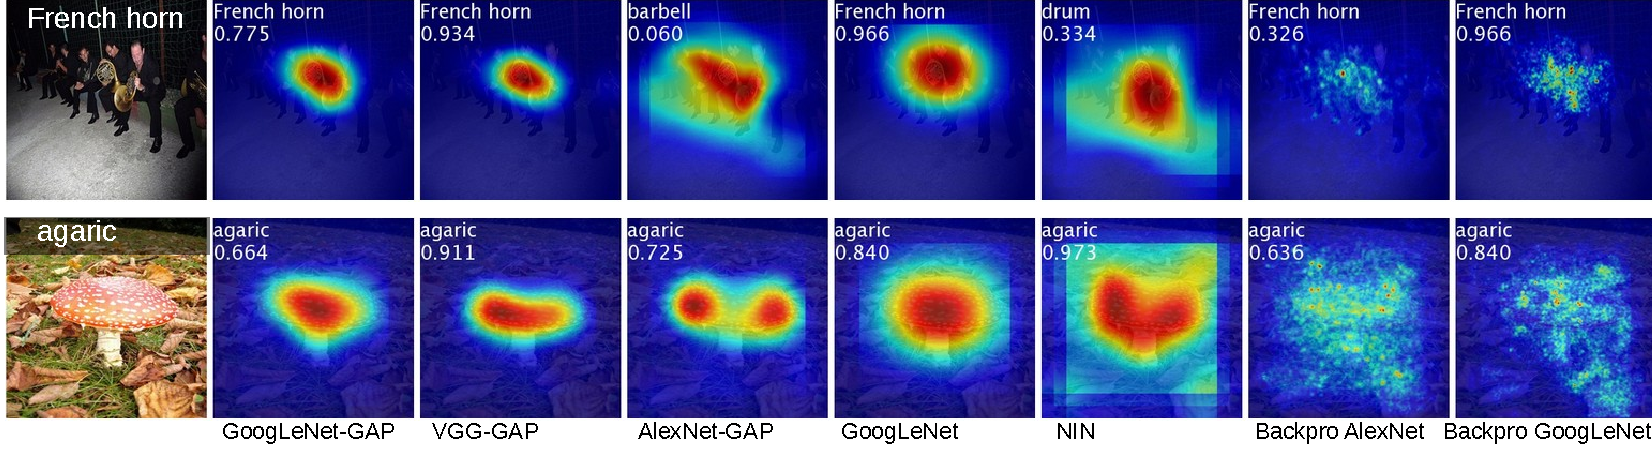
\includegraphics[width=\textwidth]{Figures/Chapter3/heatmapAll.pdf}
    \caption[Class activation maps across different architectures]{Class activation maps across different architectures: \citep{ZhouKLOT16}}
    \label{fig:cams}
\end{figure}
The drawback of their approach is, that their method can only be applied to networks which use the \texttt{GAP(Convs)} $\rightarrow$ \texttt{Fully Connected Layer (FC)} $\rightarrow$ \texttt{softmax} architecture at the end \citep{xie2020explainable}. 

\citet{SelvarajuCDVPB17} solve this impediment by generalizing CAMs to gradient-weighted class activation maps (Grad-CAMs). Since their approach only requires the final activation function to be differentiable, they are generally applicable to a broader range of CNN architectures \citep{SelvarajuCDVPB17, xie2020explainable}. For that, they compute an importance score $\Tilde{\mathbf{g}}_{\mathbf{z},c}^k$ as
\begin{equation}
\label{eq:grad_cam_importance}
     \Tilde{\mathbf{g}}_{\mathbf{z},c}^k = \frac{1}{H_\mathbf{z}W_\mathbf{z}} \sum_{i=1}^{H_\mathbf{z}} \sum_{j=1}^{W_\mathbf{z}} \frac{\partial y_c}{\partial \mathbf{z}^k_{i,j}}.
\end{equation}
Here, $y_c$ is the score before \texttt{softmax} and we calculate the gradient with respect to the feature map $\mathbf{z}^k$ in the final convolutional layer for every neuron positioned at $(i,j)$ in the $H_\mathbf{z} \times W_\mathbf{z}$ feature map \citep{SelvarajuCDVPB17, xie2020explainable}. Afterwards, these importance scores get linearly combined for every feature map as shown in \Cref{eq:grad_cam_map} where they get additionally passed through a \texttt{ReLU} function
\begin{equation}
\label{eq:grad_cam_map}
    \mathbf{M}_c = \mathtt{max}(0,\sum_{k=1}^K\Tilde{\mathbf{g}}_{\mathbf{z},c}^k \mathbf{z}^k).
\end{equation}
This computation inherently yields a $H_\mathbf{z} \times W_\mathbf{z}$ importance map ($14 \times 14$ for VGG \citep{SimonyanZ14a} and AlexNet \citep{KrizhevskySH12}, $7 \times 7$ for ResNet \citep{HeZRS16}) where we upsample it using bilinear interpolation onto the image size to yield the Grad-CAM.

Apart from CAMs, there also exist other methods like layer-wise relevance propagation \citep{MontavonLBSM17, DingLLS17, LapuschkinBMMS16, Bach2015}, deep learning important features (DeepLIFT) \citep{ShrikumarGK17}, or integrated gradients \citep{SundararajanTY17} which are not described in detail here. Please refer to \citet{xie2020explainable} or the original works for more information.

\subsubsection{Perturbation}
Perturbation methods alternate the input features to compute their respective relevance for the model's output by comparing the differences between the original and permutated version.

\citet{ZeilerF14} sweep a gray patch over the image to determine how the model will react to occluded areas. Once, an area with high correlation to the output is covered, the prediction performance drops \citep{xie2020explainable, ZeilerF14}. \citet{li2016understanding} deploy a similar idea for NLP tasks where they erase words and measure the influence on the model's performance. \citet{FongV17} define three perturbations I) replacing patches with a \emph{constant} value, II) adding \emph{noise} to a region, and  III) \emph{blurring} the area \citep{FongV17, xie2020explainable}. \citet{ZintgrafCAW17} propose a method based off \citet{Robnik-SikonjaK08} where they calculate the relevance of feature with respect to class $c$ through the prediction difference between including the respective feature or occluding it \citep{ZintgrafCAW17}. For that, they simulate the absence of each feature. A positive value for their computed difference means the feature influences the model's decision for class $c$ and a negative value means the feature influences the prediction against class $c$ \citep{ZintgrafCAW17}. \citet{ZintgrafCAW17} extend the initial method by \citet{Robnik-SikonjaK08} via removing patches instead of pixels and adapting the method for intermediate layers \citep{xie2020explainable}.

\subsection{Model distillation}
Model distillation methods allow for post-training explanations where we learn a distilled model which imitates the original model's decisions on the same data \citep{xie2020explainable}. It has access to information from the initial model and can therefore give insights about the features and output correlations \citep{xie2020explainable}. Generally, we can divide these methods into \emph{local approximation} and \emph{model translation} approaches. These either replicate the model behavior on a small subset of the input data based on the idea that the mechanisms a network uses to discriminate in a local area of the data manifold is simpler (local approximation) or stick to using the entire dataset with a smaller model (model translation) \citep{xie2020explainable}. 

\subsubsection{Local approximations}
Even though it may seem unintuitive to pursue approaches which don't explain every decision made by the DNN, practitioners often want to interpret decisions made for a specific data subset \eg employee performance indicators for those fired with poor performance \citep{xie2020explainable}. 
One of the most popular local approximations is the method proposed by \citet{Ribeiro0G16} called local interpretable model-agnostic explanations (\lime). They propose a notation where from an unexplainable global model $\modelf$ and an original representation of an instance $\xxi$ we want a interpretable model $\modelg$ from the class of potentially interpretable models $\modelg \in \gs$. Since not all models $\modelg$ have the same degree of interpretability, they define a complexity measure $\compl{\modelg}$ which could be the depth of the tree for decision trees or the number of non-zero weights in linear models \citep{Ribeiro0G16}. They incorporate this complexity measure, together with the prediction of $\modelg$ for $\modelf$ in a certain locality, in their loss term. There also exist many other works which build upon \lime{} to solve certain drawbacks  \citep{ElenbergDFK17, Ribeiro0G18}. We don't go into details here as it is only partially related to this thesis, please refer to the original works where possible.

\subsubsection{Model Translation}
The idea of \emph{model translation} is to mimic the behavior of the original deep neural network on the whole dataset, contrary to local approximations which only use a smaller subset. Some works have tried to distill neural networks into decision trees \citep{FrosstH17, tan2018learning, ZhangYMW19}, finite state automata \citep{HouZ20}, Graphs \citep{ZhangCWZ17, ZhangCSWZ18, ZhangYMW19}, or causal- and rule-based models \citep{harradon2018causal, MurdochS17}. Generally, the distilled models could be easier to deploy, faster to converge, or simply be more explainable \citep{xie2020explainable}.

\subsection{Intrinsic methods}
Finally, \emph{intrinsic} methods jointly output an explanation in combination with their prediction. In an ideal world, such methods would be on par with state-of-the-art models without explainability. This approach introduces an additional task which gets jointly trained with the original task of the model \citep{xie2020explainable}. The additional task usually tries to provide either \emph{text explanations} \citep{HindWCCDMRV19, CamburuRLB18, HendricksARDSD16, ZellersBFC19}, an \emph{explanation association} \citep{DongSZZ17, LeiBJ16, IyerLL0SS18, Alvarez-MelisJ18}, or \emph{prototypes} \citep{LiLCR18, ChenLTBRS19} which differ in the provided explainability type as well as the degree of insight. 

\subsubsection{Attention mechanism}
The \emph{attention mechanism} \citep{VaswaniSPUJGKP17} takes motivation from the human visual focus and peripheral
perception \citep{schmidt2019recurrent}. With that, humans can focus on certain regions to achieve high resolution while adjacent objects are perceived with a rather low resolution \citep{schmidt2019recurrent}. In the attention mechanism, we learn a conditional distribution over given inputs using a weighted contextual vector based off alignment scores (attention weights) \citep{xie2020explainable}. These allow for insights on how strongly different input features are considered during model inference \citep{xie2020explainable}. The alignment scores can be computed differently, for example, either content-based \citep{graves2014neural}, additive \citep{BahdanauCB14}, based on the matrix dot-product \citep{LuongPM15}, or as a scaled version of the matrix dot-product \citep{VaswaniSPUJGKP17}. Especially due to the transformer architecture \citep{VaswaniSPUJGKP17}, attention has shown to improve the neural network performance originally in natural language processing \citep{DevlinCLT19, brown2020language, lan2019albert}, but also more recently in image classification and other computer vision tasks \citep{AnwarB19, ZamirAKHK0020}. It has also been shown that attention is the update rule of a modern Hopfield network with continuous states \citep{ramsauer2020hopfield}, an architecture which hasn't been used very much in modern neural network models. Interestingly, recently there has been a discussion without clear outcome on whether or not attention counts as an explanation tool and to which degree the process actually offers insights into the inner workings of a neural network \citep{JainW19, WiegreffeP19, SenHYKR20}.

\subsubsection{Text explanations}
\emph{Text explanations} are natural language outputs which explain the model decision using a form like ``This image is of class $A$ because $B$''. As such, they are quite easy to understand regardless of the users background. Works which take this approach are, for example, \citet{HendricksARDSD16} or \citet{ParkHARSDR18}. Drawbacks of textual explanations are that they I) require supervision for explanations during training and II) explanations have been shown to be inconsistent which questions the validity of these type of explanations \citep{CamburuSMLB20}. 

\subsubsection{Explanation association}
Latent features or input elements that are combined with human-understandable concepts are classified under \emph{explanation associations}. Such explanations either combine input or latent features with semantic concepts, associate the model prediction with a set of input elements, or utilize object saliency maps \citep{xie2020explainable}.

\subsubsection{Prototypes}
\label{sec:prototypes}

Finally, model prototype approaches are specifically designed for classification tasks \citep{Bien2011, KimRS14, PriebeMDS03, wu2017prototypal}. The term \emph{prototype} in few- and zero-shot learning settings are points in the feature space representing a single class \citep{LiLCR18}. In such methods, the distance to the prototype determines how an observation is classified. The prototypes are not limited to a single observation but can also be obtained using a combination of observations or latent representations \citep{xie2020explainable}. A \emph{criticism} on the other hand, is a data instance that is not well represented by the set of prototypes \citep{molnar2019}. To obtain explainability using prototypes, one can trace the reasoning path for the prediction back to the learned prototypes \citep{xie2020explainable}. \citet{LiLCR18} use a prototype layer to deploy an explainable image classifier. They propose an architecture with an autoencoder and a prototype classifier. This prototype classifier calculates the $L^2$ distance between the encoded input and each of the prototypes, passes this through a fully connected layer to compute the sums of these distances, and finally normalizes them through a softmax layer \citep{LiLCR18}. Since these prototypes live in the same space as the encoded inputs, they can be visualized with the decoder \citep{LiLCR18}. This property, coupled with the fully connected weights, allows for explainability through visualization of the prototypes and their respective influence on the prediction. \Cref{fig:prototypes} shows the visualizations for the prototypes obtained by \citet{LiLCR18} on the MNIST \citep{lecun-mnisthandwrittendigit-2010} and Car \citep{FidlerDU12} dataset.

\begin{figure}[h]
    \centering
    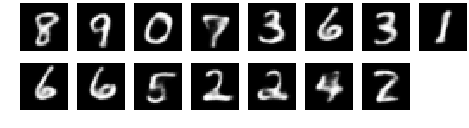
\includegraphics[width=0.49\textwidth, height=2cm]{Figures/Chapter3/prototype_result-1499.png}
    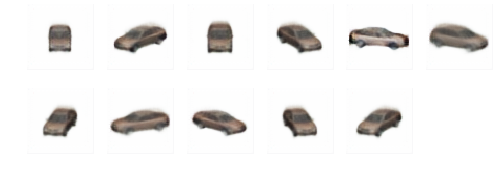
\includegraphics[width=0.4\textwidth, height=2cm]{Figures/Chapter3/car_both_R1_and_R2_new.png}
    \caption[Prototypes for the MNIST and Car dataset]{Prototypes for the MNIST (left) and Car (right) dataset: \citep{LiLCR18}}
    \label{fig:prototypes}
\end{figure}

\citet{ChenLTBRS19} introduce a prototypical part network (ProtoPNet) which has similar components to \citet{LiLCR18}, namely a convolutional neural network projecting onto a latent space and a prototype classifier. The approach chosen by \citet{ChenLTBRS19} is different as the prototypes are more fine-grained and represent parts of the input image \citep{xie2020explainable}. Hence, their model associates image patches with prototypes for explanations \citep{xie2020explainable}. \Cref{fig:looke_like} illustrates this approach for bird species classification.

\begin{figure}[h]
    \centering
    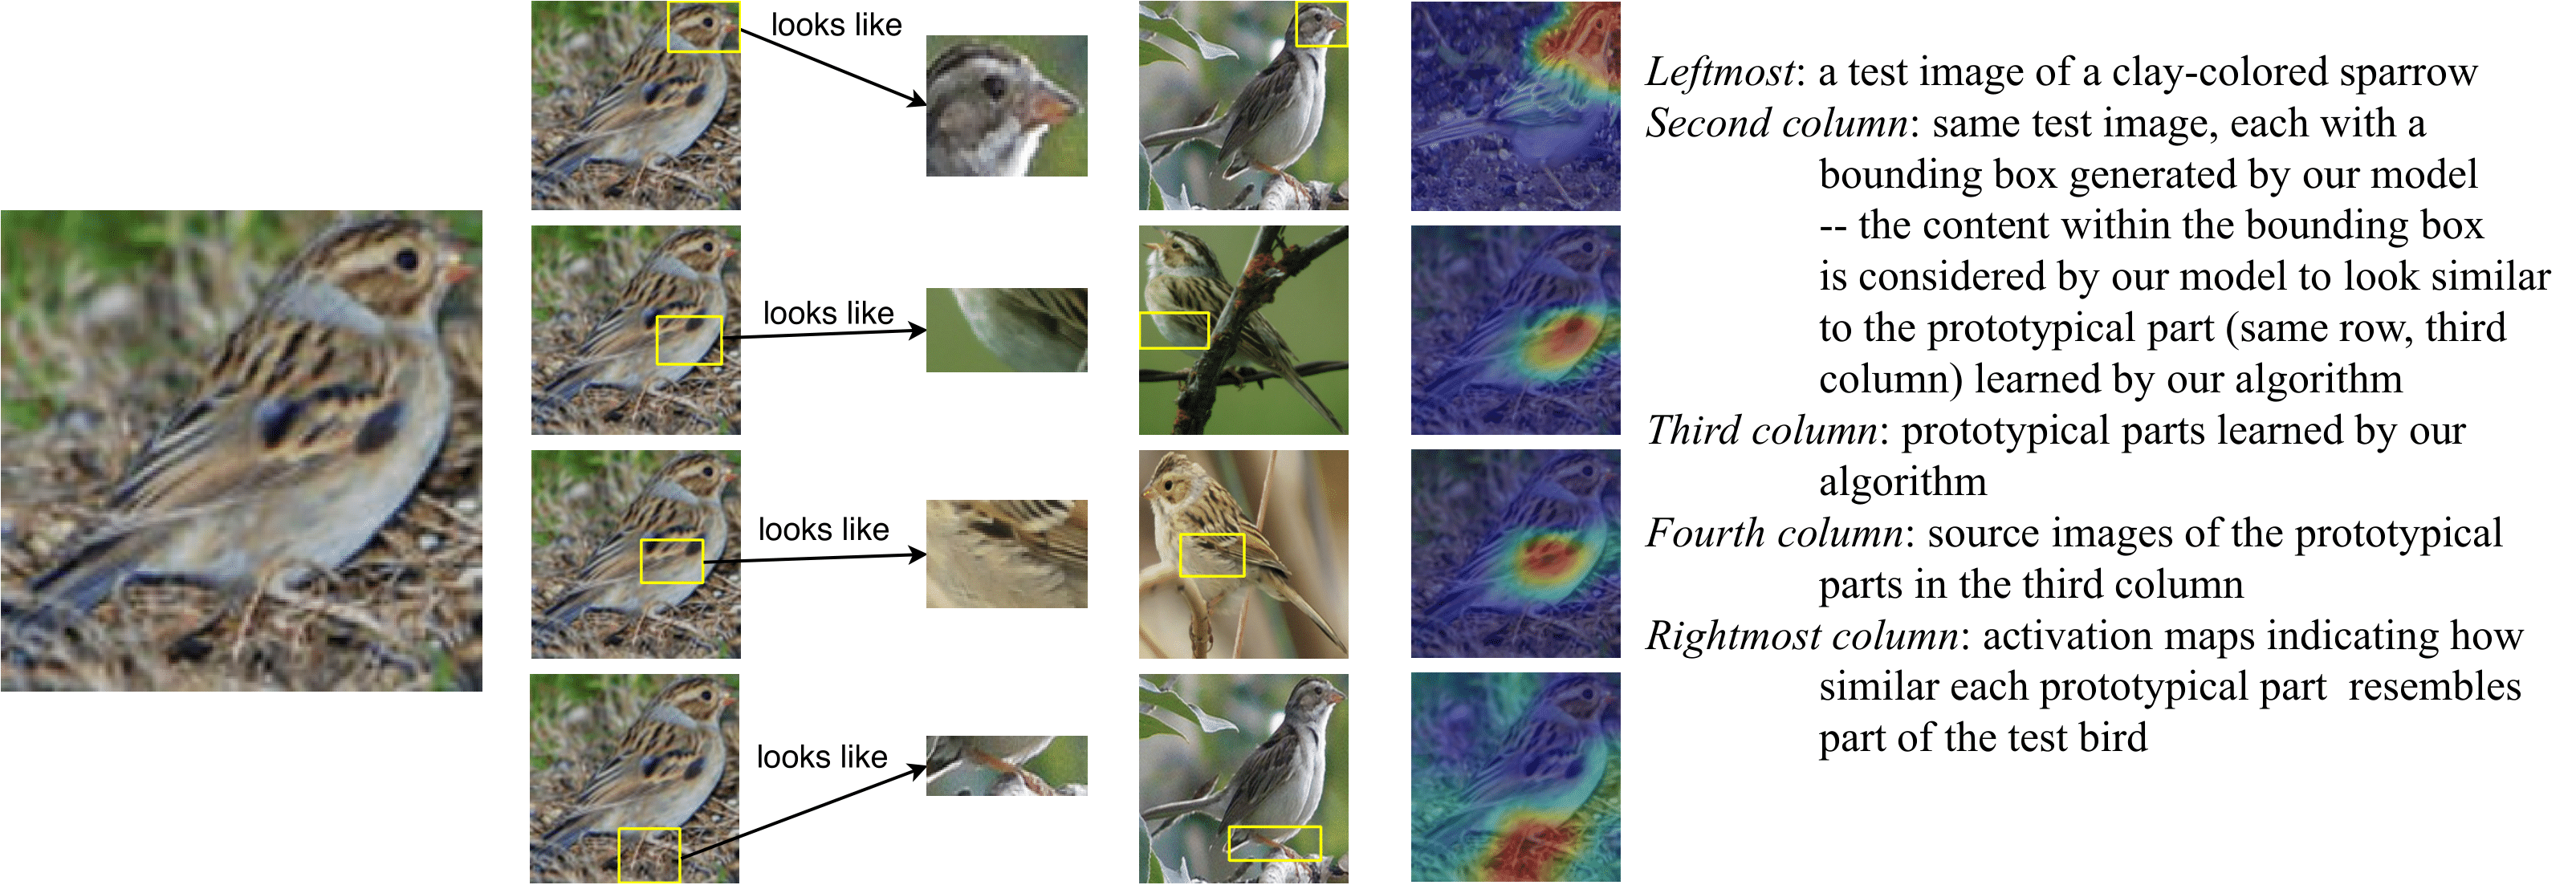
\includegraphics[width=0.95\textwidth]{Figures/Chapter3/introbird-1.png}
    \caption[Image of a clay colored sparrow and its decomposition into prototypes]{Image of a clay colored sparrow and its decomposition into prototypes: \citep{ChenLTBRS19}}
    \label{fig:looke_like}
\end{figure}
As a general framework, we would like to learn $m$ prototypes $\prots=\left\{\prot\right\}_{j=1}^{m}$ with $\prot \in \mathbb{R}^{H_{\proti} \times W_{\proti} \times K}$ which each resemble a prototypical activation pattern in a patch of the convolutional output \citep{ChenLTBRS19}. Each prototype unit $\unit$ of the prototype layer $\player$ computes \emph{some} distance metric (\eg $L^2$ norm) between the $j$-th prototype $\prot$ and all patches of $\zz$ with the same shape as $\prot$ and inverts that into a similarity score using \emph{some} mapping function \citep{ChenLTBRS19}. This computation yields a similarity map $\simmap \in \mathbb{R}^{H_\zz \times W_\zz}$ which shows how representative the $j$-th prototype is for each latent patch and this can be upsampled to the initial image size for an overlay heatmap \citep{ChenLTBRS19}. When max pooling this similarity map, we obtain a similarity score which measures how strong the $j$-th prototype is represented by \emph{any} latent patch. 

\citet{ChenLTBRS19} compute the maximum similarity score for each prototype unit $\unit$ by
\begin{equation}
\label{eq:prot_layer_function}
    \unit(\zz) = \max_{\zpatch \in \text{patches}(\zz)} \log \left( \frac{\left\|\zpatch - \prot\right\|^2_2 + 1}{\left\|\zpatch - \prot\right\|^2_2 + \stability} \right),
\end{equation}
where the squared $L^2$ distance is used and $\stability$ is a small numerical stability factor. Their modified logarithm function satisfies the property of a similarity mapping function since with an increasing $L^2$-norm the function returns a smaller value \ie larger distance values correspond to smaller similarities. Keep in mind, that this needs to be appropriately adjusted when using any other distance metric. For example, both the cosine and dot product measure have \emph{increasing} similarity values for \emph{increasing} distance values. In theory, any Bregman divergence \citep{BanerjeeMDG04} is applicable as a distance metric. However, \citet{SnellSZ17} have observed that this choice can be very impactful and the $L^2$-norm has a better performance than cosine distance for few-shot tasks. 

To enforce that every class $c$ will be represented by at least one prototype, there are a pre-determined number of prototypes for each class which is denoted as $\prots_c$ with $\prots_c \subseteq \prots$. During training, \citet{ChenLTBRS19} minimize the objective:
\begin{equation}
\label{eq:min_prototypes}
    \min_{\prots, \p_\featureex} \frac{1}{n} \sum_{i=1}^n \mathcal{L}_{\mathrm{ce}}(\underbrace{\classifier \circ \player \circ \featureex}_{\text{Prediction}\ \ypred_{i}}, \yyi) + \lambda_1 \mathcal{L}_{\mathrm{clst}} + \lambda_2 \mathcal{L}_{\mathrm{sep}},
\end{equation}
where the cluster loss $\mathcal{L}_{\mathrm{clst}}$ and separation loss $\mathcal{L}_{\mathrm{sep}}$ are defined as:
\begin{alignat}{3}
\label{eq:prototype_losses}
    \mathcal{L}_{\mathrm{clst}} &= &&\frac{1}{n} \sum_{i=1}^n \min_{j: \prot \in \prots_{\yyi}} \min_{\zpatch \in \text{patches}(\zz)} \left\|\zpatch - \prot\right\|^2_2\\
    \mathcal{L}_{\mathrm{sep}} &= -&&\frac{1}{n} \sum_{i=1}^n \min_{j: \prot \notin \prots_{\yyi}} \min_{\zpatch \in \text{patches}(\zz)} \left\|\zpatch - \prot\right\|^2_2.
\end{alignat}
Note, that this is only the first part of a multi-step training procedure where \Cref{eq:min_prototypes} solely optimizes the parameters of the featurizer $\p_\featureex$ and the prototypes $\prots$, but not the classifier as its weights $\p_w$ are frozen with an initialization for each connection $w_{c,j}$ between the $j$-th prototype unit $\unit$ and the logit for class $c$ and $\forall j: \prot \in \prots_c$ as $w_{c,j} = 1$ while $\forall j: \prot \notin \prots_c$ it is set to $w_{c,j} = -0.5$. The positive connection for the similarity to a prototype of that specific class increases the prediction value for class $c$ while the negative connection for the similarity to a prototype of a different class decreases it. This initialization, together with the separation loss, guide the prototypes to represent semantic concepts for a class, but also ensure that the same semantic concept is not learned by the other classes. Later on, \citet{ChenLTBRS19} optimize the classifier parameters $\p_\classifier$  for sparsity while fixing all other parameters to reduce the effect of \emph{negative} network reasoning for classification. 

While \citet{LiLCR18} need a decoder for visualizing the prototypes, \citet{ChenLTBRS19} don't require this component since they visualize the closest latent image patch across the full training dataset instead of directly visualizing the prototype \citep{ChenLTBRS19}. They also show that when combining several of their networks into a larger network, their method is on par with best-performing deep models \citep{ChenLTBRS19}.


\section{Explainability for Domain Generalization}

To the best of our knowledge, the only work using explanations for domain generalization is \citet{zunino2020explainable}.
They introduce a saliency based approach utilizing a 2D binary map of pixel locations for the ground-truth object segmentation as input. This map contains a $1$ in a pixel location where the class label object is present and $0$ otherwise. Even though they were able to show that their method better focuses on regions that are relevant, we identify the additional annotations of class label objects as a major drawback which we solve in this work. Indeed, we not only avoid the use of annotations by directly restoring to Grad-CAMs (see \Cref{sec:divcam}), but our idea is also different in spirit. In fact, we do not force the network to focus on relevant regions as in \cite{zunino2020explainable} but we want the network to use i) different explanations for the same objects (to achieve better generalization) and ii) the explanations to be consistent across domains (to avoid overfitting a single input distribution).